\documentclass[default]{beamer}
\setbeamertemplate{navigation symbols}{}

\usetheme{CambridgeUS}
%\useoutertheme{infolines}
\usecolortheme{beaver}

\usepackage[utf8]{inputenc}					% Выбор языка и кодировки
\usepackage[english, russian]{babel}	% Языки: русский, английский
\usepackage{csquotes}
\usepackage{tikz}
\usetikzlibrary{arrows,shapes,calc}
\usepackage{animate}
\usepackage{fp}
\usepackage{media9}
\usepackage{textpos}
\usepackage{hyperref}

\usepackage[
	language=auto,
	autolang=other,
	backend=biber,
	style=authortitle,
	sorting=ydnt,
	maxbibnames=5
]{biblatex}
\addbibresource{panov_mon.bib}
				
\DeclareSourcemap{
	\maps[datatype=bibtex, overwrite]{
		\map{
			\step[fieldset=langid, fieldvalue=english]
			\step[fieldset=doi, null]
			\step[fieldset=issn, null]
			\step[fieldset=isbn, null]
			\step[fieldset=url, null]
			\step[fieldsource=language, fieldset=langid, origfieldval]
		}
	}
}
\DeclareBibliographyDriver{std}{%
	\usebibmacro{bibindex}%
	\usebibmacro{begentry}%
	\usebibmacro{author/editor+others/translator+others}%
	\setunit{\labelnamepunct}\newblock
	\usebibmacro{title}%
	\newunit\newblock
	\usebibmacro{maintitle+booktitle}
	\newunit\newblock
	\usebibmacro{journal}%
	\newunit\newblock
	\usebibmacro{date}%
	\newunit\newblock
	\usebibmacro{finentry}
}
\DeclareBibliographyAlias{article}{std}
\DeclareBibliographyAlias{book}{std}
\DeclareBibliographyAlias{inproceedings}{std}
\DeclareBibliographyAlias{incollection}{std}

\graphicspath{{../../images/}} 			% Пути к изображениям

\makeatletter
\setbeamertemplate{footline}
{
	\leavevmode%
	\hbox{%
		\begin{beamercolorbox}[wd=.333333\paperwidth,ht=2.25ex,dp=1ex,center]{author
				in head/foot}%
			\usebeamerfont{author in
				head/foot}\insertshortauthor~~\beamer@ifempty{\insertshortinstitute}{}{(\insertshortinstitute)}
		\end{beamercolorbox}%
		\begin{beamercolorbox}[wd=.333333\paperwidth,ht=2.25ex,dp=1ex,center]{title in
				head/foot}%
			\usebeamerfont{title in head/foot}\insertshorttitle
		\end{beamercolorbox}%
		\begin{beamercolorbox}[wd=.333333\paperwidth,ht=2.25ex,dp=1ex,right]{date in
				head/foot}%
			\usebeamerfont{date in head/foot}\insertshortdate{}\hspace*{1em}
			\insertframenumber{}\hspace*{2ex} 
		\end{beamercolorbox}
	}%
	\vskip0pt%
}

\addtobeamertemplate{frametitle}{}{
	\begin{textblock*}{100mm}(\textwidth-35pt,-20pt)
		
\includegraphics[width=1.5cm]{misc/logos/frccsc.png}
	\end{textblock*}
}

\newcommand{\predmatr}[3]{
	\node[ell, rectangle, minimum height = 15, minimum width = 7.5]  at (#1 pt,#2 pt) {}; 
	\node[ellf, rectangle, minimum height = 15, minimum width = 7.5] at (#1+7.5 pt,#2 pt) {};
	\node[minimum height = 15, minimum width = 15] (#3) at (#1+3.3pt,#2 pt) {};
	\draw[ell] (#1+7.5 pt,#2+7.5 pt) -- (#1 +7.5 pt,#2-7.5 pt);
}
\renewcommand*{\bibfont}{\tiny}
\setlength\bibitemsep{-5pt}

\begin{document}
	
	\title[ИИ в образовании]{Методы искусственного интеллекта в образовании}
	\author[Панов]{Александр Игоревич Панов\\к.ф.-м.н., с.н.с.}
	\institute[ФИЦ ИУ РАН]{Отдел <<Интеллектуальные динамические системы и когнитивные исследования>>\\Институт системного анализа\\ Федеральный исследовательский центр <<Информатика и управление>>\\Российской академии наук}
	\date[23 мая]{23 мая 2018\\Семинар для сотрудников МОН РФ} 
	
	\begin{frame}
		\titlepage
		\centering
		\includegraphics[width=100pt]{misc/logos/ras.png} \hspace{10pt}
		
\includegraphics[width=80pt]{misc/logos/frccsc.png} \hspace{10pt}
		
\includegraphics[width=20pt]{misc/logos/hse.png}
	\end{frame}

	\section{Современные методы ИИ}

	\begin{frame}
		\frametitle{Кратко о себе}
		\scriptsize
		\begin{columns}
			\begin{column}{0.85\textwidth}
				\textbf{Панов Александр Игоревич, к. ф.-м. н.}
				\begin{itemize}
					\item Выпускник НГУ и МФТИ.
					\item Старший научный сотрудник отдела <<Интеллектуальные динамические системы и когнитивные исследования>> ФИЦ ИУ РАН.
					\item Научный сотрудник и доцент ФКН ВШЭ.
					\item Доцент кафедры системных исследований Московского физико-технического института (МФТИ).
					\item Член Российской ассоциации искусственного интеллекта (РААИ).
					\item Член Сообщества биологически инспирированных когнитивных архитектур (BICA Society).
					\item Участие в организации Международной конференции по биологически инспирированным когнитивным архитектурам (BICA-2016 --- Нью-Йорк, BICA-2017 --- Москва), Международной школы по биологически инспирированным когнитивным архитектурам (Fierces on BICA, Москва) и школы молодых ученых по ИИ (ISyT 2017, Санкт-Петербург).
					\item Член редколлегии журнала Biologically Inspired Cognitive Architectures.					
					\item Руководитель проектов РФФИ мол\_а, мол\_а\_дк, офи\_м.
					\item Лауреат медали РАН для молодых ученых за 2017 год.
					\item Ментор студенческой лаборатории по ИИ (SLabAI).
				\end{itemize}
			\end{column}
			
			\begin{column}{0.15\textwidth}
				\centering
				\includegraphics[width=\textwidth]{misc/logos/ras.png}
				\vspace{7pt}
				
\includegraphics[width=\textwidth]{misc/logos/frccsc.png}
				\vspace{7pt}
				\includegraphics[width=0.7\textwidth]{misc/logos/isa.png}
				\vspace{7pt}
				\includegraphics[width=0.5\textwidth]{misc/logos/raai.png}
				\vspace{7pt}
				
\includegraphics[width=0.5\textwidth]{misc/logos/hse.png}
				\vspace{7pt}
				\includegraphics[width=\textwidth]{misc/logos/mipt.jpg}
				\vspace{5pt}
				\includegraphics[width=\textwidth]{misc/logos/BICA.png}
				\vspace{5pt}
				\includegraphics[width=0.7\textwidth]{misc/logos/slabai3.png}
			\end{column}
			
		\end{columns}
	\end{frame}

	\begin{frame}
		\frametitle{Искусственный интеллект и когнитивные науки}
		
		\centering
		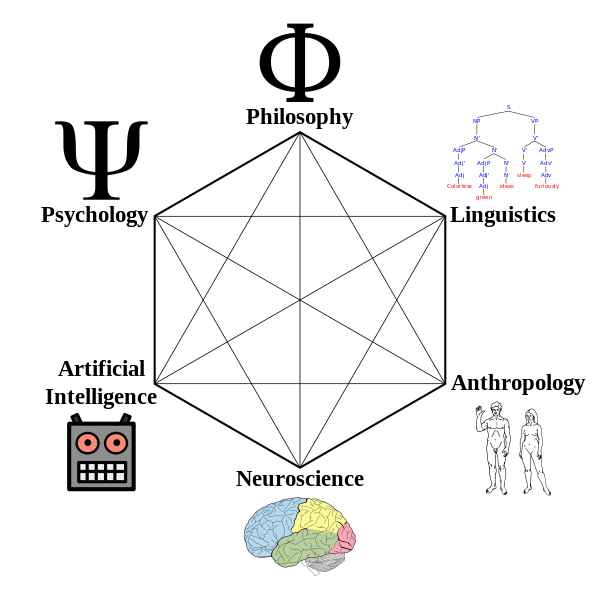
\includegraphics[width=0.5\textwidth]{cogsci.png}
	\end{frame}
	
	\begin{frame}
		\frametitle{Основные направления ИИ}
		\centering
		\footnotesize
		\makebox[0.8\textwidth][c]{
			\begin{tikzpicture}
			\node[ellipse, minimum width = 100, minimum height = 50, fill=blue!20, align=center] (d1) {Искусственный\\интеллект};
			
			\node[rounded corners=5pt,draw,color=blue!20, very thick,text=black] (d2) at (-4,2) {
				\begin{minipage}[c][33pt]{100pt}
				\centering
				\textbf{Приобретение знаний, анализ данных и порождение гипотез}
				\end{minipage}
			};
			\node[rounded corners=5pt,draw,color=blue!20, very thick,text=black] (d3) at (-4,0.5) {
				\begin{minipage}[c][20pt]{80pt}
				\centering
				\textbf{Моделирование рассуждений}
				\end{minipage}
			};
			
			\node[rounded corners=5pt,draw,color=blue!20, very thick,text=black] (d4) at (-4,-0.7) {
				\begin{minipage}[c][20pt]{80pt}
				\centering
				\textbf{Многоагентные системы}
				\end{minipage}
			};
			
			\node[rounded corners=5pt,draw,color=blue!20, very thick,text=black] (d5) at (-4,-2.3) {
				\begin{minipage}[c][43pt]{110pt}
				\centering
				\textbf{Обработка естественного языка, пользовательский интерфейс и модели пользователя}
				\end{minipage}
			};
			
			
			\node[rounded corners=5pt,draw,color=blue!20, very thick,text=black] (d6) at (4,2) {
				\begin{minipage}[c][33pt]{120pt}
				\centering
				\textbf{Динамические интеллектуальные системы и планирование поведения}
				\end{minipage}
			};
			\node[rounded corners=5pt,draw,color=blue!20, very thick,text=black] (d7) at (4,0.5) {
				\begin{minipage}[c][20pt]{80pt}
				\centering
				\textbf{Представление знаний}
				\end{minipage}
			};
			
			\node[rounded corners=5pt,draw,color=blue!20, very thick,text=black] (d8) at (4,-0.7) {
				\begin{minipage}[c][20pt]{100pt}
				\centering
				\textbf{Нечеткие модели и мягкие вычисления}
				\end{minipage}
			};
			
			\node[rounded corners=5pt,draw,color=blue!20, very thick,text=black] (d9) at (4,-2.3) {
				\begin{minipage}[t][20pt]{110pt}
				\centering
				\textbf{Инструментальные средства и технологии}
				\end{minipage}
			};
			
			\draw[->,rounded corners=10pt, very thick, blue!20](d1)[xshift=-10] |- (d2.east);
			\draw[->,rounded corners=10pt, very thick, blue!20](d1)[xshift=10] |- (d6.west);
			
			\draw[->,rounded corners=10pt, very thick, blue!20](d1)[xshift=-10] |- (d5.east);
			\draw[->,rounded corners=10pt, very thick, blue!20](d1)[xshift=10] |- (d9.west);
			
			\draw[->,rounded corners=10pt, very thick, blue!20](d1) |- (d3.east);
			\draw[->,rounded corners=10pt, very thick, blue!20](d1) |- (d7.west);
			
			\draw[->,rounded corners=10pt, very thick, blue!20](d1.south west) |- (d8.west);
			\draw[->,rounded corners=10pt, very thick, blue!20](d1.south east) |- (d4.east);
			\end{tikzpicture}
		}
				
		\nocite{*}
		\printbibliography[keyword={osipovai}, resetnumbers=true]
		
	\end{frame}

	
	\section{Нейронные сети и когнитивные науки}				
	\begin{frame}
		\frametitle{Нейронные сети "--- графы вычислений}
		\centering
		\animategraphics[loop,controls,width=0.3\linewidth]{25}{tensor-}{0}{207}
		\vspace{-5pt}
		\nocite{*}
		\printbibliography[keyword={tensor}, resetnumbers=true]
	\end{frame}

	\begin{frame}
		\frametitle{Нейронные сети "--- графы вычислений}
		\centering
		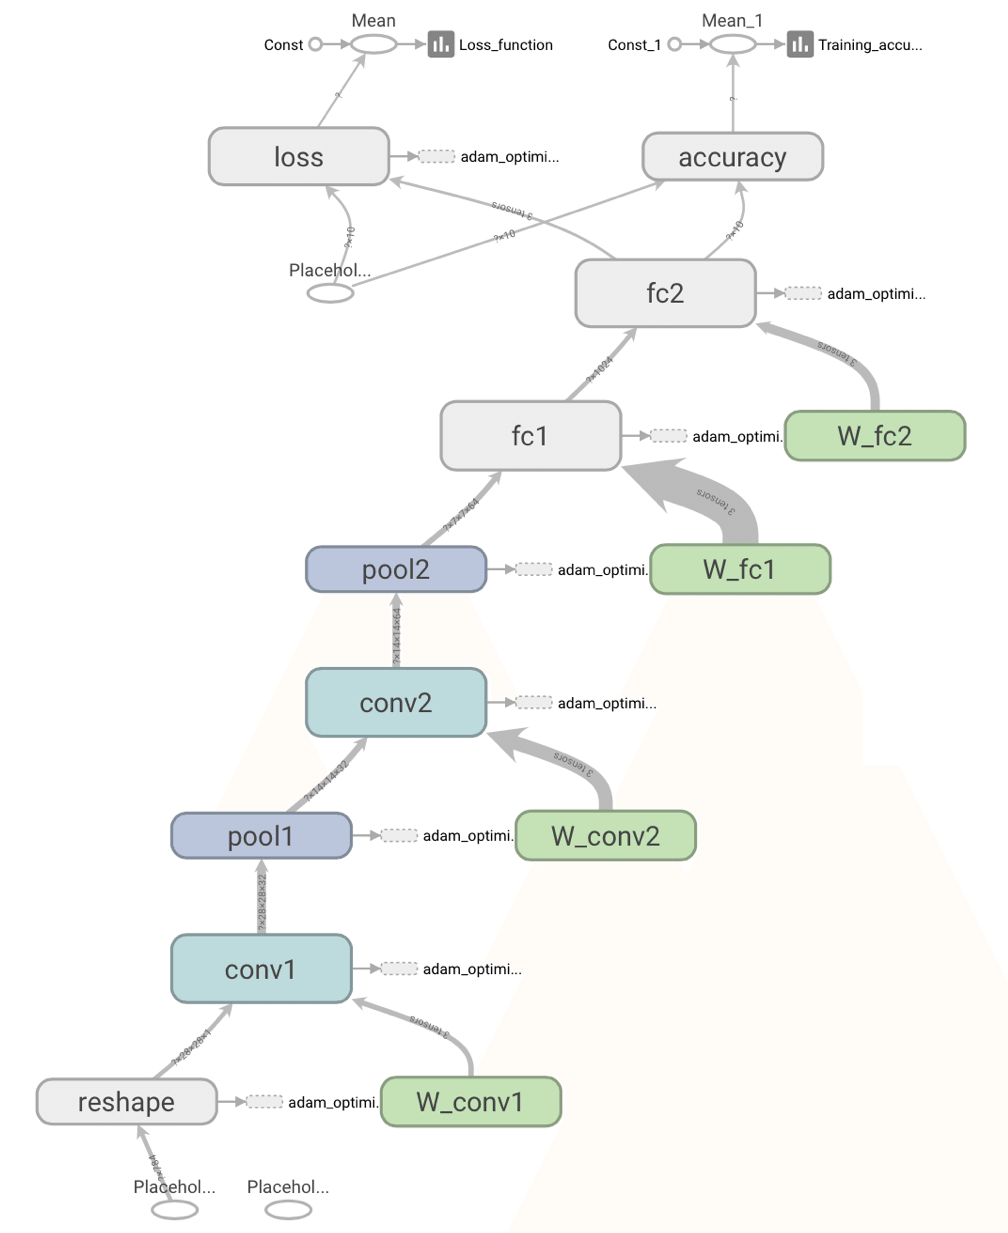
\includegraphics[width=0.5\linewidth]{graphs.png}
	\end{frame}

	\begin{frame}
		\frametitle{Нейронный субстрат}
		
		\begin{columns}
			\begin{column}{0.35\textwidth}
				\includegraphics[width=0.8\textwidth]{misc/phisio/mozg_2}
				\par\bigskip
				\hspace{-7mm}\includegraphics[width=\textwidth]{misc/phisio/mozg}
			\end{column}
			\begin{column}{0.65\textwidth}
				\includegraphics[width=\textwidth]{misc/phisio/cortex_layers}
			\end{column}
		\end{columns}
		\nocite{*}
		\printbibliography[keyword={column}, resetnumbers=true]
	\end{frame}
		
		
	\begin{frame}
		\frametitle{Гетерархическая модель}
		\scriptsize
		Расширенная реализация иерархической временной памяти (hierarchical temporal memory - HTM) - \textbf{гетерархическая каузальная сеть (heterarchical causal network - HCN)}.
		
		\begin{center}
		\includegraphics[width=0.4\textwidth]{misc/mpf/hawkins_htm}
		\end{center}
		\nocite{*}
		\printbibliography[keyword={starthtm}, resetnumbers=true]
	\end{frame}
		
	\begin{frame}
		\frametitle{Гетерархическая модель}
		
		\begin{center}
		\includegraphics[width=0.3\textwidth]{misc/mpf/hawkins_htm_ex_a}
		\includegraphics[width=0.3\textwidth]{misc/mpf/hawkins_htm_ex_b}
		\end{center}
		\nocite{*}
		\printbibliography[keyword={hetermem}, resetnumbers=true]
	\end{frame}
		
	\begin{frame}
		\frametitle{Нейронная организация}
		
		\begin{columns}
		\begin{column}{0.65\textwidth}
		\includegraphics[width=0.9\textwidth]{misc/mpf/regions_connect}
		\end{column}
		\begin{column}{0.35\textwidth}
		\includegraphics[width=\textwidth]{misc/phisio/column}
		\end{column}
		\end{columns}
		\nocite{*}
		\printbibliography[keyword={simplehtm}, resetnumbers=true]
	\end{frame}
	
	\begin{frame}
		\frametitle{Спайковые модели}
		
		\begin{center}
			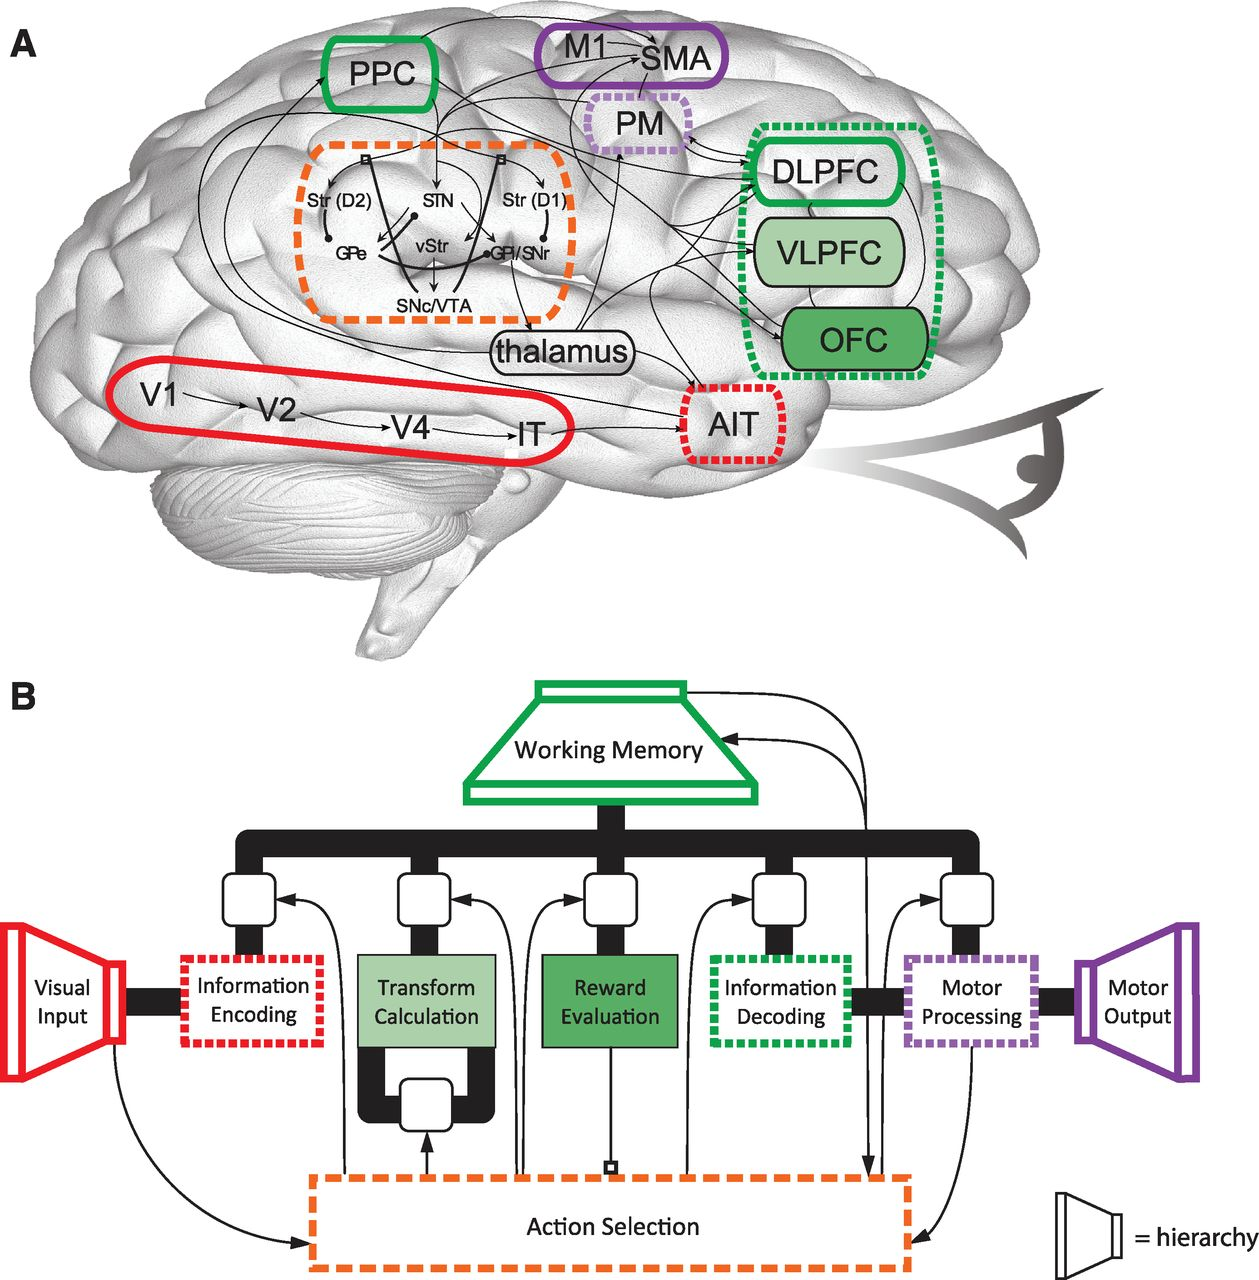
\includegraphics[width=0.5\textwidth]{spaun.jpeg}
		\end{center}
				
		\nocite{*}
		\printbibliography[keyword={spawn}, resetnumbers=true]
	\end{frame}

	\begin{frame}
		\frametitle{Когнитивные архитектуры}
		
		\begin{center}
			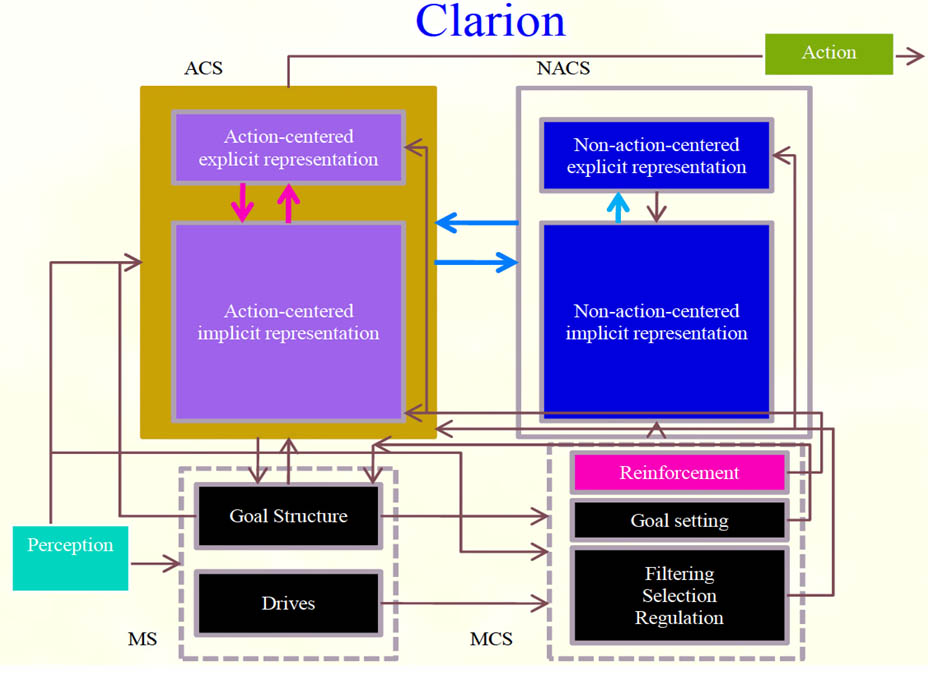
\includegraphics[width=0.45\textwidth]{clarion.jpg}
			
			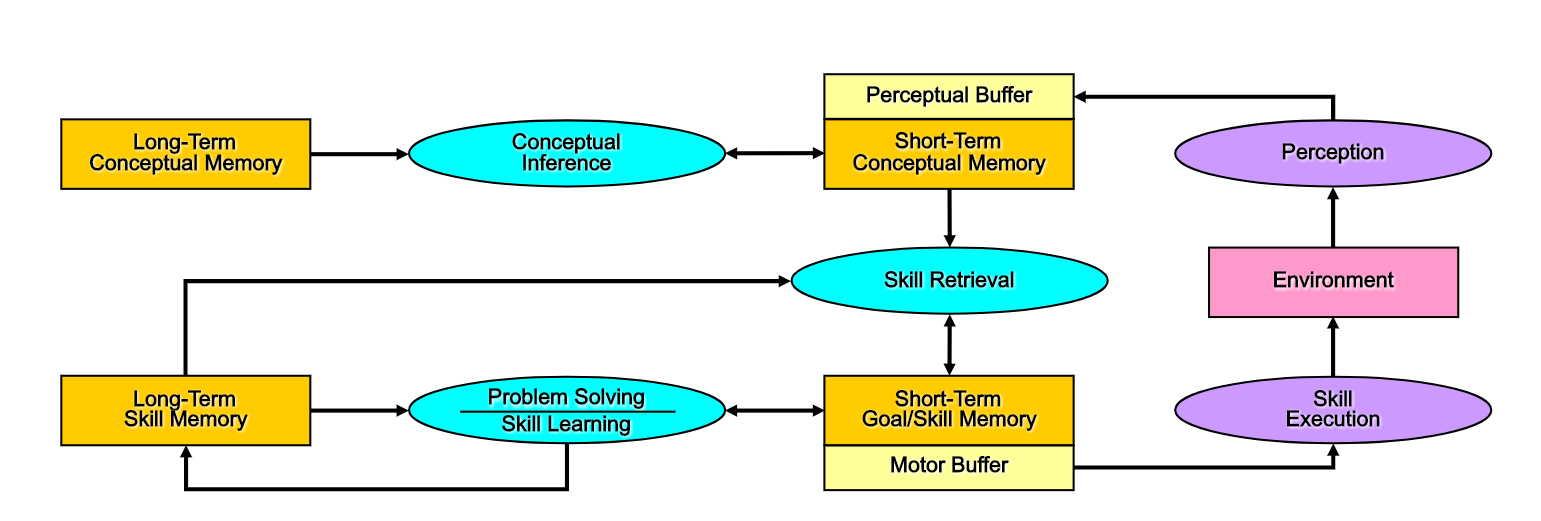
\includegraphics[width=0.5\textwidth]{icarus.png}
		\end{center}
		
		\vspace{-5pt}
		\nocite{*}
		\printbibliography[keyword={symbgrnd}, resetnumbers=true]
	\end{frame}

	\begin{frame}
		\frametitle{Сравнение: текущая ситуация}
		
		\begin{itemize}
			\item У ИНС и ЕНС совершенно различны принципы структурной организации (послойность и гетерархия).
			\item У ИНС и ЕНС совершенно различны принципы обучения и адаптации (градиентные методы и правила Хебба).
			\item Перспектива - в разработке биологически правдоподобных подходов (кортикоморфных и спайковых).
		\end{itemize}
	\end{frame}
	
	\section{Применение ИИ в образовании}
	
	\begin{frame}
		\frametitle{ИТ и ИИ в образовании "--- EdTech}
		
		Основная задача, которая ставится в EdTech - это \textbf{адаптация} образовательного процесса и материалов под \textbf{индивидуальные особенности} обучающегося и преподавателя. Основные заказчики - системы online-обучения (Stepik, Logiclike, Examer, Skyeng, Lingualeo).

		\centering
		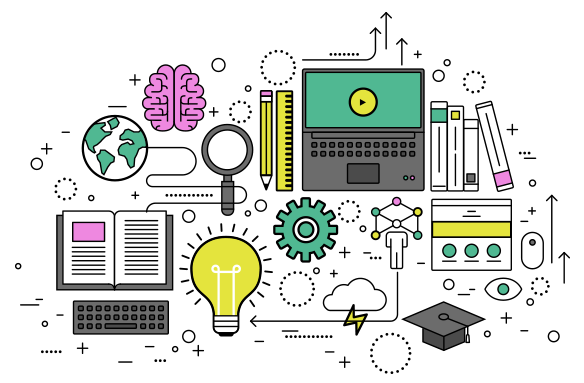
\includegraphics[width=\textheight]{edtech.png}
		
	\end{frame}
	
	
	\begin{frame}
		\frametitle{Направления в EdTech}
	
		\begin{itemize}
			\item Динамический порядок блоков курса.
			\item Генерация FAQ - ответов на часто задаваемые вопросы.
			\item Прокторинг - отслеживание поведения обучающегося во время занятия.
			\item Автоматическая проверка домашних заданий, контрольных и т.п.
			\item Интерактивное информирование преподавателя о степени усвоения материала.
			\item Рекомендации преподавателю о том, как лучше подавать материал.
		\end{itemize}
	
		\begin{center}
			
\includegraphics[height=0.2\textheight]{techno.png}
			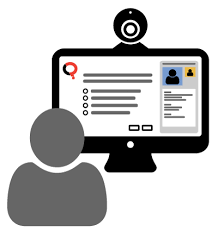
\includegraphics[height=0.2\textheight]{proctoring.png}
			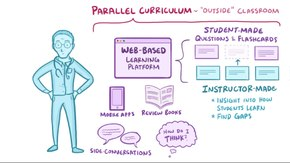
\includegraphics[height=0.2\textheight]{adaptive.jpg}
		\end{center}
		
		\begin{tiny}
			\color{blue}
			How AI Impacts Education - \href{https://www.forbes.com/sites/theyec/2017/12/27/how-ai-impacts-education}{Forbse}
			
			Artificial Intelligence: Implications for the Future of Education - \href{http://www.gettingsmart.com/2018/01/artificial-intelligence-implications-for-the-future-of-education/}{Gettings Smart}
			
			Искусственный интеллект в образовании: в поисках сферы применения - \href{http://robotoved.ru/ai_education_russia/}{Роботовед}
		\end{tiny}
	\end{frame}
	
	\section{Перспективные направления}
	
	\begin{frame}
		\frametitle{Когнитивный ассистент}
		
		
			\begin{columns}
				\begin{column}{0.7\textwidth}
					Работает в нескольких режимах:
					\begin{itemize}
						\item диалог на свободную тему (chit-chat),
						\item вопросно-ответный режим,
						\item целеориентированный режим, в нашем случае в области образования.
					\end{itemize}
				\end{column}
				\begin{column}{0.3\textwidth}
					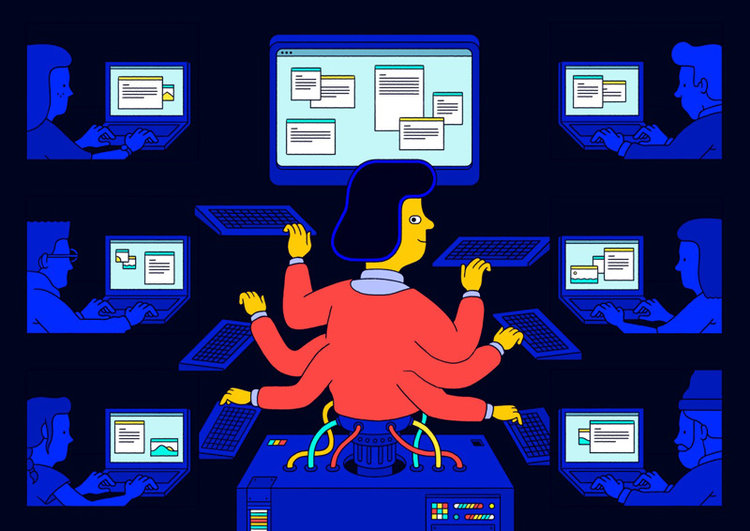
\includegraphics[width=0.9\textwidth]{assistant.jpg}
				\end{column}
			\end{columns}

		\begin{itemize}
			\item Имеет свою картину мира, описывающую его назначение, цели, возможные действия и сценарии, личностные смыслы, оценки достижения целей.
			\item Персонифицированный: сроит в процессе общения картину мира собеседника, выявляет его сценарии и личностные смыслы, ценности, предпочтения, привычки и т.п.
			\item Проактивный: сам инициирует взаимодействие, напоминает о необходимости действий с учётом картины мира собеседника.
			\item Понимает русский язык
		\end{itemize}
	\end{frame}

	\begin{frame}
		\frametitle{Картина мира субъекта деятельности}
		\scriptsize
		\onslide<1->{
			Картина мира субъекта деятельности - это представления субъекта о внешней среде, о своих собственных характеристиках, целях, мотивах, о других субъектах и операции (произвольные и непроизвольные), осуществляемые на основе этих представлений.
		}
		\onslide<2->{
			\par\smallskip
			Элементом картины мира является знак:
			\begin{itemize}
				\item в смысле культурно-исторического подхода Выготского-Лурии,
				\item выполняющий функции в соответствии с теорией деятельности Леонтьева.
			\end{itemize}
		}
		\onslide<3->{
			\begin{columns}
				\begin{column}{0.4\textwidth}
					\centering
					\includegraphics[width=0.6\textwidth]{signs/ru/sign_color_book_ru}
				\end{column}
			}
			\onslide<4->{
				\begin{column}{0.6\textwidth}
					\begin{columns}
						\begin{column}{0.5\textwidth}
							\centering
							\includegraphics[width=\textwidth]{misc/phisio/ivan_cyrc}
						\end{column}
						\begin{column}{0.5\textwidth}
							\centering
							\includegraphics[width=\textwidth]{misc/phisio/workspace}
						\end{column}
					\end{columns}
					
				\end{column}
			\end{columns}
			В пользу существования такой структуры свидетельствуют:
			\begin{itemize}
				\item нейрофизиологические данные (Эдельман, Иваницкий, Маунткастл и др.),
				\item другие психологические теории (например, трехкомпонентная модель Станович).
			\end{itemize}
			\vspace{-5pt}
			\nocite{*}
			\printbibliography[keyword={sign}, resetnumbers=true]
		}
	\end{frame}

	\begin{frame}
		\frametitle{Три образующих элемента картины мира}
		\footnotesize
		\begin{figure}
		\includegraphics[width=0.3\textwidth]{signs/ru/sign_colored}
		\end{figure}
		
		Представляемая сущность описывается тремя причинно-следственными (каузальными) структурами:
		\begin{itemize}
		\item {\color{red}структура образа} - представление взаимосвязи внешних сигналов и внутренних характеристик субъекта (агента) - сенсо-моторное представление,
		\item {\color{blue}структура значения} - обобщенное знание о соотношениях во внешнем мире, согласованное в некоторой группе субъектов (агентов),
		\item {\color{green!60!black}структура личностного смысла} - ситуационная потребностно-мотивационная интерпретация знаний о соотношениях во внешней среде (значение для себя).
		\end{itemize}
		\nocite{*}
		\printbibliography[keyword={qualia}, resetnumbers=true]
	\end{frame}
	
	\begin{frame}
		\frametitle{Реляционно-ситуационный анализ текста}
		\begin{center}
			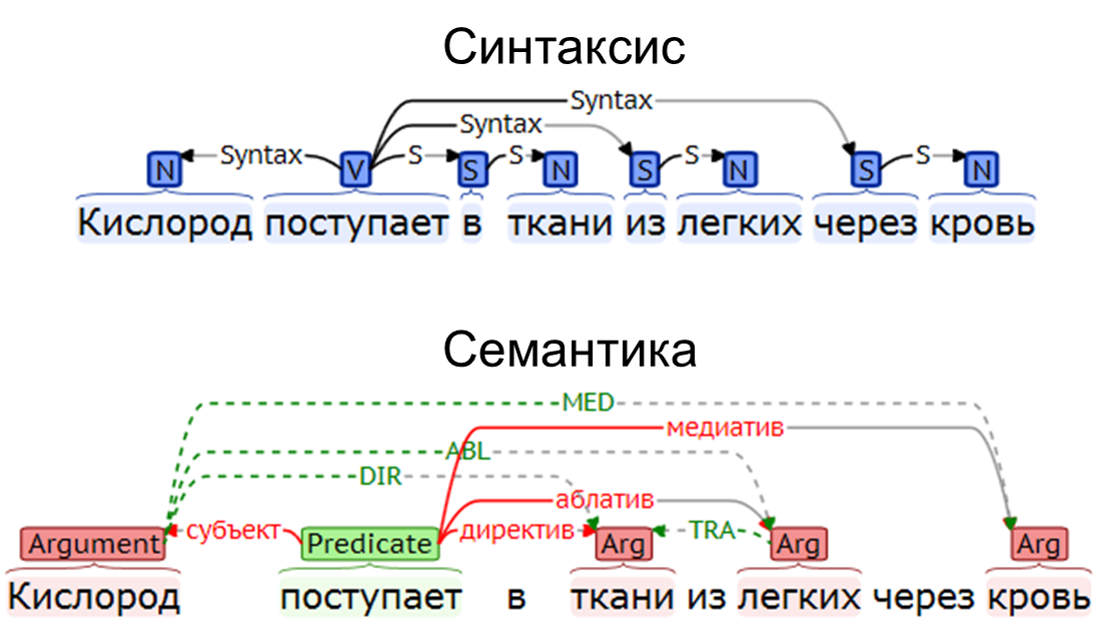
\includegraphics[width=0.8\textwidth]{nlp.png}
		\end{center}
		
		
		\begin{tiny}
			\color{blue}
			Сервис по анализу текста - \href{http://nlp.isa.ru}{ФИЦ ИУ РАН}
			
		\end{tiny}
	\end{frame}
	
	\section{Заключение}
	
	\begin{frame}
		\frametitle{Вопросы семинара}
		
		\begin{itemize}
			\item Можно ли перенести накопленный опыт по обучению нейронных сетей на методы обучения естественных нейронных сетей - {\color{red} нет}. Напрямую, без <<психологических>> методов, в настоящее время это не возможно.
			\item Каковы перспективы использования такого опыта в образовании - {\color{red} мозг-компьютер интерфейс}. Более перспективным, с целью приобретения, а не <<вживление>> знаний, является когнитивный ассистент.
		\end{itemize}
	\end{frame}
	\begin{frame}
		\centering
		\Huge
		Спасибо за внимание!
		\normalsize
		\par\bigskip
		\par\bigskip
		\par\bigskip
		Панов Александр Игоревич
		
		pan@isa.ru
	\end{frame}			
\end{document}
	
	
